<<<<<<< HEAD
\documentclass{article}

\usepackage{microtype}
\usepackage{amsmath}
\usepackage{enumitem}
\usepackage{etoolbox}
\usepackage[svgnames]{xcolor}
\usepackage{pgfplots}
\usepackage{tikz}
\usepackage[letterpaper]{geometry}

\pgfplotsset{compat=newest}

\newcommand{\diff}[1]{\frac{#1}{dt}}
\newcommand{\vel}{\mathrm{v}}
\newcommand{\x}{\mathrm{x}}
\newcommand{\inter}{\int_{t_1}^{t_2}}
\newcommand{\tvert}{\biggr\rvert_{t_1}^{t_2}}
\newcommand{\derv}{\frac{\mathrm{d}}{\mathrm{d}t}}
\newcommand{\ddx}{\frac{\mathrm{d}}{\mathrm{d}x}}

\patchcmd\subequations
 {\theparentequation\alph{equation}}
 {\subequationsformat}
 {}{}

\newcommand{\subequationsformat}{\theparentequation.\arabic{equation}}

\author{Laith}
\title{Introduction to Physics}
\date{1/25/2023}

\begin{document}
	\maketitle
	\section{What is Physics?}
	Physics is the study of how the objects around us change over time. 
	This includes their \textbf{position}, \textbf{displacement}, \textbf{distance}, and \textbf{speed}.
	\subsection{Position}
	The \textbf{position} of an object is its relative distance from a reference point. For example, if we had a red dot and a green dot on a line, then we could
	determine the position of the red dot to be its distance from the green dot and the position of the green dot to be its distance from the red dot.
	We can express position as a function $\mathrm{x(t)}$.
	\subsection{Displacement}
	\textbf{Displacement} is the difference between an objects new position and its previous position. If we had a red dot move from point 1 to point 2, then the
	displacement of the red dot would be the difference in position of point 2 and point 1.
	Mathematically, we can represent this as $\Delta{x}$.
	\[\Delta{x} = x_2-x_1\]
	Since position is a function, $x_2$ and $x_1$ can be written as $x(t_2)$ and $x(t_1)$, where $t_2$ is the time at which
	the object was at position 2 and $t-1$ is the time at which the object was at position 1. Thus, we can write 
	displacement as:
	\[\Delta{x} = \mathrm{x(t_2)}-\mathrm{x(t_1)}\]  
	\subsection{Distance}
	\textbf{Distance} is the length of the path traveled by an object from one point to another.
	\subsection{Speed}
	\textbf{Speed} is how fast an object moved from one point to another. As an extension, \textbf{velocity} is just speed, but in specific direction. In other words,
	speed is a \emph{scalar}, velocity is a \emph{vector}, but both represent how fast an object moves. The rate at which velocity change over time is known as \textbf{acceleration}.
	We can represent velocity as a function $\mathrm{v(t)}$. We could try to define this function as the ratio between displacement and time elapsed between two points:
	\[\overline{\mathrm{v(t)}} = \frac{\Delta{x}}{\Delta{t}}\]
	The issue with this equation is that velocity can change at any given time, thus in order to get closer to a true representation
	of velocity, we need to look at instantaneous intervals of velocity. In other words: we differentiate position.
	\[\mathrm{v(t)} = \diff{dx}\]
	By differentiating position, we will get the rate at which position changes at a specific time $t$, which is the velocity at that specific time.
	\subsection{Acceleration}
	\textbf{Acceleration} is the rate at which the velocity of an object changes, however with a few exceptions,
	we will assume acceleration to be constant for the majority of this course. Thus, we will represent
	acceleration as a variable $a$, and if acceleration is not constant, a function $\mathrm{a(t)}$.

	Since acceleration is the rate at velocity changes, we can differentiate velocity to get acceleration:
	\[\mathrm{a} = \diff{dv}\]
	This also means that if we want to get velocity, but only have acceleration, we can integrate acceleration to get
	velocity:
	\begin{align*}
	\mathrm{v(t)\biggr\rvert_{t_1}^{t_2}} & = \int_{t_2}^{t_1}a\,dt\\
	\mathrm{v(t)\biggr\rvert_{t_1}^{t_2}} & = a\cdot t\biggr\rvert_{t_1}^{t_2}\\
	\mathrm{v(t)\biggr\rvert_{t_1}^{t_2}} & = a\cdot t_2 - a \cdot t_1 = a\cdot (t_2-t_1)\\
	\mathrm{v(t_2)-v(t_1)} & = a\cdot(t_2 - t_1)
	\end{align*}
	\section{Time}
	Objects always move with respect to time, as the definition of physics would imply. Thus, we treat time as an independant variable; while position, displacement,
	distance, speed, velocity, and acceleration are all functions of time.
	\section{Problems}
	\subsection{The Rabbit}
	A rabbit is moving along a straigh line. At time $t_1=0$ the raddit is distance $x_1=1\mathrm{m}$ from your right
	and is moving towards the right with a velocity of $v_1=1\mathrm{\frac{m}{s}}$. The rabbit has a constant acceleration
	of $a=1\mathrm{\frac{m}{s^2}}$ towards the right. What is the position of the rabbit as time $t_2=10s$?
	\subsubsection{Solution}
	First we list our known variables followed by our unknowns:
	\begin{align*}
	&\mathrm{\underline{Knowns}}\\
	&x_1 =1\mathrm{m} \\
	&t_1 =0\mathrm{s}\\
	&v_1 =1\mathrm{\frac{m}{s}} \\
	&t_2 = 10\mathrm{s}\\
	&a =1\mathrm{\frac{m}{s^2}}\\
	&\mathrm{\underline{Unknowns}}\\
	&x_2 = ?\\
	&v_2 = ?
	\end{align*}
	Then we illustrate the scenario:
	\begin{figure}[hh]
	\begin{center}
	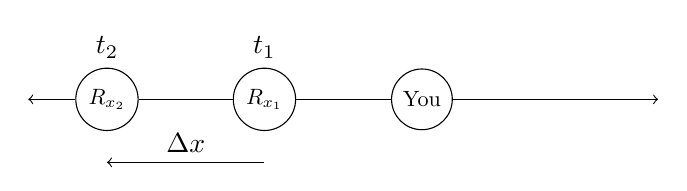
\begin{tikzpicture}
		\node[above] at (3, 0.4) (t1) {$t_1$};
		\node[above] at (1, 0.4) (t2) {$t_2$};
		\node[circle, draw, scale=0.8] at (3, 0) (r) {$R_{x_1}$};
		\node[circle, draw, scale=0.8] at (1, 0) (r2) {$R_{x_2}$};
		\node[circle, draw, scale=0.8] at (5, 0) (y) {You};

		\draw[<-] (0, 0) -- (r2);
		\draw (r2) -- (r);
		\draw (r) -- (y);
		\draw[->] (y) -- (8, 0);

		\node[above] at (2, -0.8) (x) {$\Delta{x}$};

		\draw[<-] (1, -0.8) -- (3, -0.8);
	\end{tikzpicture}
	\end{center}
    \end{figure}
	% \newpage
	While we do know velocity at time $t=0\mathrm{s}$, we do not know velocity at time $t=10\mathrm{s}$.
	We don't need to know the value of velocity at this point, it will give us the grounds to define an expression
	for $\mathrm{v(t)}$, which we can differentiate to get a function for position, allowing us to calculate the final
	position of the rabbit.

	Since we know acceleration $a=1\mathrm{\frac{m}{s^2}}$, including the fact that it is constant, we can
	differentiate acceleration to find a function for velocity:
	\begin{subequations}
	\begin{align}
		a &= \diff{dv}\\
		\int_{t_2}^{t_1}a\,dt &= \int_{t_2}^{t_1}\diff{dv}\\
		a\cdot t\biggr\rvert_{t_1}^{t_2} &= \mathrm{v}(t) \biggr\rvert_{t_1}^{t_2}\\
		&\Rightarrow \mathrm{v}(t_2)-\mathrm{v}(t_1) = a\cdot(t_2 - t_1)\\
		&\Rightarrow \mathrm{v}(t_2) = a\cdot (t_2-t_1) + \mathrm{v}(t_1)
	\end{align}
	Now that we have a function for velocity, we can utilize the fact that velocity
	is the derivative of position, allowing us to set our function equal to $dx$:
	\[\diff{dx} = \mathrm{v}(t_2) = a\cdot(t_2-t_1)+\mathrm{v}(t_1)\]
	We can now omit $\mathrm{v}(t_2)$ since we aren't looking for it, giving us a clean equation that we
	can integrate to get the value of $x_2$. Naturally, we want to integrate with the upper limit 
	$t_2$ and the lower limit $t_1$:
	\begin{align}
		\int_{t_1}^{t_2} \diff{dx}\,dt &= \int_{t_1}^{t_2} [a\cdot (t_2-t_1) + v_1] \,dt\\
		\int_{t_1}^{t_2}\diff{dx}\,dt &= \int_{t_1}^{t_2} a\cdot(t_2-t_1)\,dt + \int_{t_1}^{t_2} v_1\,dt\\
		\mathrm{x}(t)\biggr\rvert_{t_1}^{t_2} &= \int_{t_1}^{t_2}(a\cdot \Delta{t}) \,dt + (v_1\cdot t) \biggr\rvert_{t_1}^{t_2}\\
		\mathrm{x}(t)\biggr\rvert_{t_1}^{t_2} &= a\frac{\Delta{t}^2}{2} \biggr\rvert_{t_1}^{t_2} + (v_1\cdot t) \biggr\rvert_{t_1}^{t_2}
	\end{align}
	Note: $\Delta{t} = t - t_1$ where $t$ is a parameter.
	\begin{align}
		\mathrm{x}(t_2)-\mathrm{x}(t_1) &= a(\frac{\Delta{t}^2(t_2)}{2} - \frac{\Delta{t}^2(t_1)}{2}) + v_1\cdot (t_2-t_1)\\
		\mathrm{x}(t_2)-\mathrm{x}(t_1) &= a(\frac{(t_2-t_1)^2}{2} - \frac{(t_1-t_1)^2}{2}) + v_1\cdot (t_2-t_1)\\
		\mathrm{x}(t_2) &= a(\frac{(t_2-t_1)^2}{2} - \frac{(t_1-t_1)^2}{2}) + v_1\cdot (t_2-t_1) + \mathrm{x}(t_1)\\
		x_2 &= a(\frac{(t_2-t_1)^2}{2} - \frac{(t_1-t_1)^2}{2}) + v_1\cdot (t_2-t_1) + x_1\\
	\end{align}
	We now have an equation for $x_2$. Now all we need to do now is plug in our knowns.
	\begin{align}
		x_2 &= (1)(\frac{(10-0)^2}{2} - \frac{(0-0)^2}{2}) + (1)\cdot (10-0) + (1)\\
		x_2 &= 1(\frac{(10)^2}{2} - \frac{(0)^2}{2}) + 1\cdot 10 + 1\\
		x_2 &= 1(\frac{100}{2} - \frac{0}{2}) + 10 + 1\\
		x_2 &= 1(50 - 0) + 11\\
		x_2 &= 50 + 11\\
		x_2 &= 61\\
	\end{align}
	\end{subequations}
	Our answer: $61\mathrm{m}$. The final position of the rabbit (the position of the rabit at
	time $t_2=10\mathrm{s}$) is $61$ meters from our right.
	\subsection{The Police Car and the Speeding Car}
	A car is moving with a constant speed $v$. It passes a police car on the side of the road.
	The officer realized that the speed of the car was over the limit and starts to chase it at
	time $t=10\,\mathrm{s}$ after the car passed by. The police car moves with a constant acceleration 
	of $a=10\,\mathrm{m/s^2}$ and reaches the car at $t=30\,\mathrm{s}$. What is the velocity of the
	speeding car?
	\subsubsection{Solution}
	Lets draw the scenario:
	\begin{figure}[hh]
	\begin{center}
	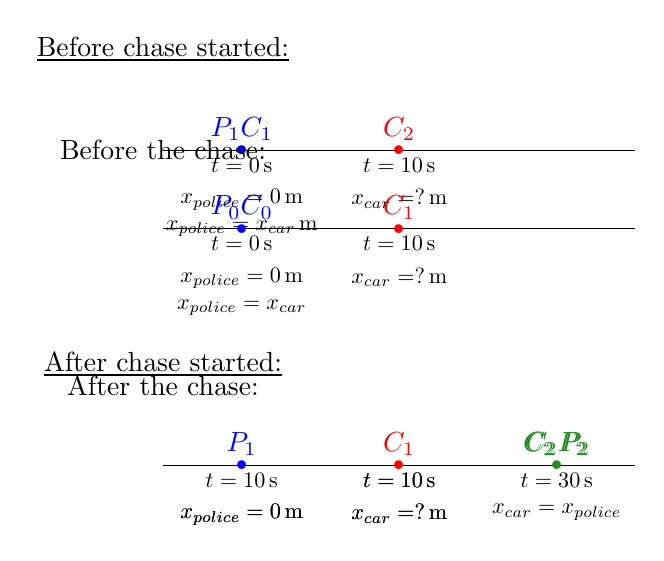
\begin{tikzpicture}
<<<<<<< HEAD
		\node[above] at (-1, 5) {\underline{Before chase started:}};
		\draw[] (-1, 4) -- (5, 4);

		\node[above, scale=1, color=blue] at (0, 4) (p) {$P_1C_1$};
		\node[above, scale=1, color=red] at (2, 4) (c) {$C_2$};

		\node[scale=3, color=blue] at (0, 4) (p1) {.};
		\node[scale=3, color=red] at (2, 4) (p2) {.};
		
		\node[below, scale=0.8] at (0, 4) (p) {$t=0\,\mathrm{s}$};
		\node[below, scale=0.8] at (2, 4) (c) {$t=10\,\mathrm{s}$};
		\node[below, scale=0.8] at (2, 4-0.4) (x) {$x_{car}=?\,\mathrm{m}$};
		\node[below, scale=0.8] at (0, 4-0.4) (x) {$x_{police}=0\,\mathrm{m}$};
		\node[below, scale=0.8] at (0, 4-0.8) (x) {$x_{police}=x_{car}\,\mathrm{m}$};

		\node[above] at (-1, 1) {\underline{After chase started:}};
=======
		\node at (-1, 4) {\text{Before the chase:}};
		\draw[] (-1, 3) -- (5, 3);

		\node[above, scale=1, color=blue] at (0, 3) (p) {$P_0C_0$};
		\node[above, scale=1, color=red] at (2, 3) (c) {$C_1$};

		\node[scale=3, color=blue] at (0, 3) (p1) {.};
		\node[scale=3, color=red] at (2, 3) (p2) {.};
		
		\node[below, scale=0.8] at (0, 3) (p) {$t=0\,\mathrm{s}$};
		\node[below, scale=0.8] at (2, 3) (c) {$t=10\,\mathrm{s}$};
		\node[below, scale=0.8] at (2, 3-0.4) (x) {$x_{car}=?\,\mathrm{m}$};
		\node[below, scale=0.8] at (0, 3-0.4) (x) {$x_{police}=0\,\mathrm{m}$};
		\node[below, scale=0.8] at (0, 3-0.8) (x) {$x_{police}=x_{car}$};

		\node at (-1, 1) {\text{After the chase:}};
>>>>>>> 5f7ec571d8ab143d7344b6729df45392af8d3ea0
		\draw[] (-1, 0) -- (5, 0);

		\node[above, scale=1, color=blue] at (0, 0) (p) {$P_1$};
		\node[above, scale=1, color=red] at (2, 0) (c) {$C_1$};
<<<<<<< HEAD
		\node[above, scale=1, color=ForestGreen] at (4, 0) (x) {$C_2\,P_2$};
=======
		\node[above, scale=1, color=ForestGreen] at (4, 0) (x) {$C_2P_2$};
>>>>>>> 5f7ec571d8ab143d7344b6729df45392af8d3ea0

		\node[scale=3, color=blue] at (0, 0) (p1) {.};
		\node[scale=3, color=red] at (2, 0) (p2) {.};
		\node[scale=3, color=ForestGreen] at (4, 0) (p3) {.};
		
		\node[below, scale=0.8] at (0, 0) (p) {$t=10\,\mathrm{s}$};
<<<<<<< HEAD
		\node[below, scale=0.8] at (2, 0) (c) {$t=10\,\mathrm{s}$};
		\node[below, scale=0.8] at (2, -0.4) (x) {$x_{car}=?\,\mathrm{m}$};
		\node[below, scale=0.8] at (0, -0.4) (x) {$x_{police}=0\,\mathrm{m}$};
=======
		\node[below, scale=0.8] at (0, -0.4) (x) {$x_{police}=0\,\mathrm{m}$};
		\node[below, scale=0.8] at (2, 0) (c) {$t=10\,\mathrm{s}$};
		\node[below, scale=0.8] at (2, -0.4) (x) {$x_{car}=?\,\mathrm{m}$};
>>>>>>> 5f7ec571d8ab143d7344b6729df45392af8d3ea0
		\node[below, scale=0.8] at (4, 0) (x) {$t=30\,\mathrm{s}$};
		\node[below, scale=0.8] at (4, -0.4) (x) {$x_{car}=x_{police}$};
	\end{tikzpicture}
	\end{center}
    \end{figure}

<<<<<<< HEAD
	Lets list our known and unknown variables:
	\begin{align*}
		&\mathrm{\underline{Knowns}}\\
		&t_1 =0\,\mathrm{s} \\
		&t_2 = 30\,\mathrm{s} \\
		&{v_1}_{police} =0\,\mathrm{m/s} \\
		&a_{police} =10\,\mathrm{m/s^2}\\
		&\x_{police}(0) = \x_{police}(10) = 0\,\mathrm{m}\\
		&a_{car} =0\,\mathrm{m/s^2}\\
		&\mathrm{\underline{Unknowns}}\\
		&{x_1}_{car} = ?\\
		&x_2 = ?\\
		&{v_2}_{police} = ?\\
		&{v}_{car} = ?
	\end{align*}

	\paragraph{Setting up the Math} We will make the position of the police car at time $t=0$ our
	reference position. Since the position of the speeding car is equal to that of the police car at 
	time $t=0$, we can say that $\x_{car}(0)=0$. We can also set $t_1=0$ and $t_2=30$, in which both cars
	meet at time $t=30$ and start at the same position at time $t=0$. We will be integrating with respect to 
	time, in which our limits will be $a=t_1$ and $b=t_2$.

	Since the cars meet 30 seconds into the scenario, we can set up the below equation:
	\[\x_{car}(30) = \x_{police}(30)\]
	Naturally, we will need to find an expression for each function, and we can do so by integrating accelerations.

	We can determine the acceleration of the speeding car in two ways:
	\begin{enumerate}[label=(\alph*)]
		\item Differentiating velocity.
		\item Making a logical deduction.
	\end{enumerate}

	With approach \textbf{a}, we know that the differentiating velocity will give us the acceleration of the speeding car,
	and we also know that the velocity of the speeding car is constant.
	By differentiating a constant, we will get $0$:
	\[a = \ddx v_{car} = \ddx C = 0\]
	Thus, our acceleration $a$ is $0\,\mathrm{m/s^2}$


	\begin{subequations}	
=======
	We can even take a closer look by roughly graphing the positions of the car with 
	respect to time:
	\begin{center}
		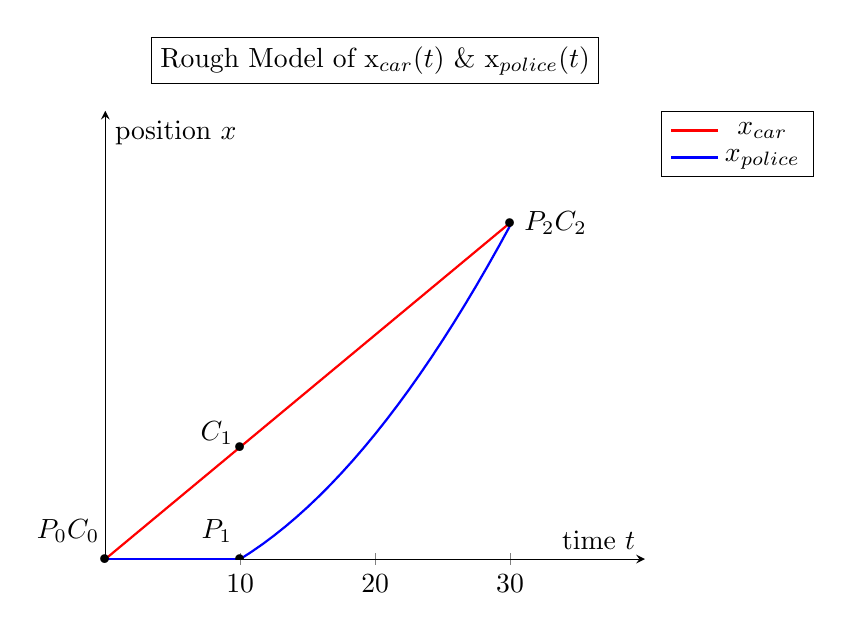
\begin{tikzpicture}
			\begin{axis}
				[
					domain=0:40,
					xmin=0,
					xmax=40,
					ymax=40,
					axis lines=center,
					legend pos=outer north east,
					title=$\boxed{\text{Rough Model of }\x_{car}(t)\text{ \& }\x_{police}(t)}$,
					xlabel=time $t$,
					ylabel=position $x$,
					xtick={0, 10, 20, 30},
					ytick,
				]
				\addplot[no marks, thick, domain=0:30, color=red] {x};
				\addlegendentry{$x_{car}$};
				\addplot[no marks, thick, domain=0:10, color=blue] {0};
				\addplot[no marks, thick, domain=10:30, color=blue] {(1/26.9)*(x-10)*(x+10)};
				\addlegendentry{$x_{police}$};

				\node[scale=3] at (30, 30) (x) {.};
				\node[right of=x, xshift=-12] {$P_2C_2$};
				\node[scale=3] at (10, 10) (x1) {.};
				\node[left of=x1, xshift=20, yshift=5] {$C_1$};
				\node[scale=3] at (10, 0) (x2) {.};
				\node[left of=x2, xshift=20, yshift=10] {$P_1$};
			\end{axis}
				\node[scale=3] at (0, 0) (x3) {.};
				\node[left of=x3, xshift=15, yshift=10] {$P_0C_0$};
		\end{tikzpicture}
	\end{center}

	From the graph, we can see that the speeding car moves for the entirety of the chase whereas
	the police car only begins to move $10$ seconds into the chase. We can also see that both cars 
	are at the same position at time $t=0$ and $t=30$, and so this will be our reference position. 
	As a result, we will set $t_2=30$ for both cars, but $t_1=0$ for the speeding car and $t_1=10$
	for the police car.
	
	Since the positions of both cars are equal at $t_2$, we can say that:
	\[\x_{car}(t_2) = \x_{police}(t_2) \]
	Now, while we know that $t_2=30$, we still need a expression for each function.

	\paragraph{The Police Car} In order define $\x_{police}(t)$, we need to integrate the velocity
	of the police car, however we do not have a velocity. Thus, we have to integrate acceleration to 
	get velocity, and we are given a constant acceleration of $a=10$:

	\begin{subequations}
	\begin{align}
		\vel_{car}(t) &= \int_{t_1}^{t} a \,\mathrm{d}t \\
		\vel_{car}(t) &= \int_{t_1}^{t} 10\,\mathrm{d}t \\
		\vel_{car}(t) &= [10(t) + C] - [10(t_1) + C]\\
		\vel_{car}(t) &= 10(t) - 10(10)\\
		\vel_{car}(t) &= 10t - 100 \\
	\end{align}
	Now to derive the function for position:
	\begin{align}
		\x_{car}(t) &= \int_{t_1}^{t} \vel_{car}(t)\,\mathrm{d}t \\
		\x_{car}(t) &= \int_{t_1}^{t} 10t - 100 \,\mathrm{d}t \\
		\x_{car}(t) &= [10\frac{(t)^2}{2}-100t+C] - [10\frac{(t_1)^2}{2}-100t+C] \\
		\x_{car}(t) &= [10\frac{(t)^2}{2}-100t] - [10\frac{(10)^2}{2}-100(10)]\\
		\x_{car}(t) &= 5t^2-100t - (-500)\\
		\x_{car}(t) &= 5t^2 - 100t + 500 \\
	\end{align}

	\paragraph{The Speeding Car} We will have to integrate velocity to derive a function
	for the speeding car's position, however while we do not know the value of its velocity,
	we can just take the integral of a constant:
	\begin{align}
		\x_{car}(t) &= \int_{t_1}^{t} v_{car} \\
		\x_{car}(t) &= t\cdot v_{car} - t_1\cdot v_{car} \\
		\x_{car}(t) &= t\cdot v_{car} - (0)\cdot v_{car} \\
		\x_{car}(t) &= t\cdot v_{car}
	\end{align}

	\newpage
	Now to set the two functions equal to each other at $t=t_2=30$:
	\begin{align}
		\x_{car}(30) &= \x_{police}(30) \\
		30\cdot v_{car} &= 5(30)^2 - 100(30) + 500 \\
		30\cdot v_{car} &= 2000 \\
		\Rightarrow v_{car} &= \frac{2000}{30} \\
		&\boxed{v_{car} = \frac{200}{3} \,\mathrm{m/s}}
	\end{align}	
>>>>>>> 5f7ec571d8ab143d7344b6729df45392af8d3ea0
	\end{subequations}
	Thus, the velocity of the speeding car was $\frac{200}{3}\,\mathrm{m/s}$.
\end{document}
=======
\documentclass{article}

\usepackage{microtype}
\usepackage{amsmath}
\usepackage{enumitem}
\usepackage{etoolbox}
\usepackage[svgnames]{xcolor}
\usepackage{pgfplots}
\usepackage{tikz}
\usepackage[letterpaper]{geometry}

\pgfplotsset{compat=newest}

\newcommand{\diff}[1]{\frac{#1}{dt}}
\newcommand{\vel}{\mathrm{v}}
\newcommand{\x}{\mathrm{x}}
\newcommand{\inter}{\int_{t_1}^{t_2}}
\newcommand{\tvert}{\biggr\rvert_{t_1}^{t_2}}
\newcommand{\derv}{\frac{\mathrm{d}}{\mathrm{d}t}}

\patchcmd\subequations
 {\theparentequation\alph{equation}}
 {\subequationsformat}
 {}{}

\newcommand{\subequationsformat}{\theparentequation.\arabic{equation}}

\author{Laith}
\title{Introduction to Physics}
\date{1/25/2023}

\begin{document}
	\maketitle
	\section{What is Physics?}
	Physics is the study of how the objects around us change over time. 
	This includes their \textbf{position}, \textbf{displacement}, \textbf{distance}, and \textbf{speed}.
	\subsection{Position}
	The \textbf{position} of an object is its relative distance from a reference point. For example, if we had a red dot and a green dot on a line, then we could
	determine the position of the red dot to be its distance from the green dot and the position of the green dot to be its distance from the red dot.
	We can express position as a function $\mathrm{x(t)}$.
	\subsection{Displacement}
	\textbf{Displacement} is the difference between an objects new position and its previous position. If we had a red dot move from point 1 to point 2, then the
	displacement of the red dot would be the difference in position of point 2 and point 1.
	Mathematically, we can represent this as $\Delta{x}$.
	\[\Delta{x} = x_2-x_1\]
	Since position is a function, $x_2$ and $x_1$ can be written as $x(t_2)$ and $x(t_1)$, where $t_2$ is the time at which
	the object was at position 2 and $t-1$ is the time at which the object was at position 1. Thus, we can write 
	displacement as:
	\[\Delta{x} = \mathrm{x(t_2)}-\mathrm{x(t_1)}\]  
	\subsection{Distance}
	\textbf{Distance} is the length of the path traveled by an object from one point to another.
	\subsection{Speed}
	\textbf{Speed} is how fast an object moved from one point to another. As an extension, \textbf{velocity} is just speed, but in specific direction. In other words,
	speed is a \emph{scalar}, velocity is a \emph{vector}, but both represent how fast an object moves. The rate at which velocity change over time is known as \textbf{acceleration}.
	We can represent velocity as a function $\mathrm{v(t)}$. We could try to define this function as the ratio between displacement and time elapsed between two points:
	\[\overline{\mathrm{v(t)}} = \frac{\Delta{x}}{\Delta{t}}\]
	The issue with this equation is that velocity can change at any given time, thus in order to get closer to a true representation
	of velocity, we need to look at instantaneous intervals of velocity. In other words: we differentiate position.
	\[\mathrm{v(t)} = \diff{dx}\]
	By differentiating position, we will get the rate at which position changes at a specific time $t$, which is the velocity at that specific time.
	\subsection{Acceleration}
	\textbf{Acceleration} is the rate at which the velocity of an object changes, however with a few exceptions,
	we will assume acceleration to be constant for the majority of this course. Thus, we will represent
	acceleration as a variable $a$, and if acceleration is not constant, a function $\mathrm{a(t)}$.

	Since acceleration is the rate at velocity changes, we can differentiate velocity to get acceleration:
	\[\mathrm{a} = \diff{dv}\]
	This also means that if we want to get velocity, but only have acceleration, we can integrate acceleration to get
	velocity:
	\begin{align*}
	\mathrm{v(t)\biggr\rvert_{t_1}^{t_2}} & = \int_{t_2}^{t_1}a\,dt\\
	\mathrm{v(t)\biggr\rvert_{t_1}^{t_2}} & = a\cdot t\biggr\rvert_{t_1}^{t_2}\\
	\mathrm{v(t)\biggr\rvert_{t_1}^{t_2}} & = a\cdot t_2 - a \cdot t_1 = a\cdot (t_2-t_1)\\
	\mathrm{v(t_2)-v(t_1)} & = a\cdot(t_2 - t_1)
	\end{align*}
	\section{Time}
	Objects always move with respect to time, as the definition of physics would imply. Thus, we treat time as an independant variable; while position, displacement,
	distance, speed, velocity, and acceleration are all functions of time.
	\section{Problems}
	\subsection{The Rabbit}
	A rabbit is moving along a straigh line. At time $t_1=0$ the raddit is distance $x_1=1\mathrm{m}$ from your right
	and is moving towards the right with a velocity of $v_1=1\mathrm{\frac{m}{s}}$. The rabbit has a constant acceleration
	of $a=1\mathrm{\frac{m}{s^2}}$ towards the right. What is the position of the rabbit as time $t_2=10s$?
	\subsubsection{Solution}
	First we list our known variables followed by our unknowns:
	\begin{align*}
	&\mathrm{\underline{Knowns}}\\
	&x_1 =1\mathrm{m} \\
	&t_1 =0\mathrm{s}\\
	&v_1 =1\mathrm{\frac{m}{s}} \\
	&t_2 = 10\mathrm{s}\\
	&a =1\mathrm{\frac{m}{s^2}}\\
	&\mathrm{\underline{Unknowns}}\\
	&x_2 = ?\\
	&v_2 = ?
	\end{align*}
	Then we illustrate the scenario:
	\begin{figure}[hh]
	\begin{center}
	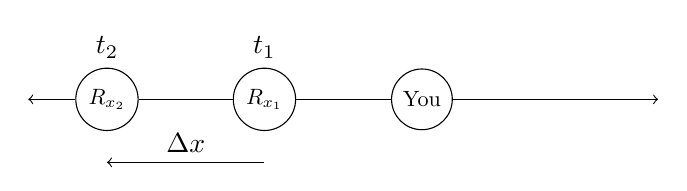
\begin{tikzpicture}
		\node[above] at (3, 0.4) (t1) {$t_1$};
		\node[above] at (1, 0.4) (t2) {$t_2$};
		\node[circle, draw, scale=0.8] at (3, 0) (r) {$R_{x_1}$};
		\node[circle, draw, scale=0.8] at (1, 0) (r2) {$R_{x_2}$};
		\node[circle, draw, scale=0.8] at (5, 0) (y) {You};

		\draw[<-] (0, 0) -- (r2);
		\draw (r2) -- (r);
		\draw (r) -- (y);
		\draw[->] (y) -- (8, 0);

		\node[above] at (2, -0.8) (x) {$\Delta{x}$};

		\draw[<-] (1, -0.8) -- (3, -0.8);
	\end{tikzpicture}
	\end{center}
    \end{figure}
	% \newpage
	While we do know velocity at time $t=0\mathrm{s}$, we do not know velocity at time $t=10\mathrm{s}$.
	We don't need to know the value of velocity at this point, it will give us the grounds to define an expression
	for $\mathrm{v(t)}$, which we can differentiate to get a function for position, allowing us to calculate the final
	position of the rabbit.

	Since we know acceleration $a=1\mathrm{\frac{m}{s^2}}$, including the fact that it is constant, we can
	differentiate acceleration to find a function for velocity:
	\begin{subequations}
	\begin{align}
		a &= \diff{dv}\\
		\int_{t_2}^{t_1}a\,dt &= \int_{t_2}^{t_1}\diff{dv}\\
		a\cdot t\biggr\rvert_{t_1}^{t_2} &= \mathrm{v}(t) \biggr\rvert_{t_1}^{t_2}\\
		&\Rightarrow \mathrm{v}(t_2)-\mathrm{v}(t_1) = a\cdot(t_2 - t_1)\\
		&\Rightarrow \mathrm{v}(t_2) = a\cdot (t_2-t_1) + \mathrm{v}(t_1)
	\end{align}
	Now that we have a function for velocity, we can utilize the fact that velocity
	is the derivative of position, allowing us to set our function equal to $dx$:
	\[\diff{dx} = \mathrm{v}(t_2) = a\cdot(t_2-t_1)+\mathrm{v}(t_1)\]
	We can now omit $\mathrm{v}(t_2)$ since we aren't looking for it, giving us a clean equation that we
	can integrate to get the value of $x_2$. Naturally, we want to integrate with the upper limit 
	$t_2$ and the lower limit $t_1$:
	\begin{align}
		\int_{t_1}^{t_2} \diff{dx}\,dt &= \int_{t_1}^{t_2} [a\cdot (t_2-t_1) + v_1] \,dt\\
		\int_{t_1}^{t_2}\diff{dx}\,dt &= \int_{t_1}^{t_2} a\cdot(t_2-t_1)\,dt + \int_{t_1}^{t_2} v_1\,dt\\
		\mathrm{x}(t)\biggr\rvert_{t_1}^{t_2} &= \int_{t_1}^{t_2}(a\cdot \Delta{t}) \,dt + (v_1\cdot t) \biggr\rvert_{t_1}^{t_2}\\
		\mathrm{x}(t)\biggr\rvert_{t_1}^{t_2} &= a\frac{\Delta{t}^2}{2} \biggr\rvert_{t_1}^{t_2} + (v_1\cdot t) \biggr\rvert_{t_1}^{t_2}
	\end{align}
	Note: $\Delta{t} = t - t_1$ where $t$ is a parameter.
	\begin{align}
		\mathrm{x}(t_2)-\mathrm{x}(t_1) &= a(\frac{\Delta{t}^2(t_2)}{2} - \frac{\Delta{t}^2(t_1)}{2}) + v_1\cdot (t_2-t_1)\\
		\mathrm{x}(t_2)-\mathrm{x}(t_1) &= a(\frac{(t_2-t_1)^2}{2} - \frac{(t_1-t_1)^2}{2}) + v_1\cdot (t_2-t_1)\\
		\mathrm{x}(t_2) &= a(\frac{(t_2-t_1)^2}{2} - \frac{(t_1-t_1)^2}{2}) + v_1\cdot (t_2-t_1) + \mathrm{x}(t_1)\\
		x_2 &= a(\frac{(t_2-t_1)^2}{2} - \frac{(t_1-t_1)^2}{2}) + v_1\cdot (t_2-t_1) + x_1\\
	\end{align}
	We now have an equation for $x_2$. Now all we need to do now is plug in our knowns.
	\begin{align}
		x_2 &= (1)(\frac{(10-0)^2}{2} - \frac{(0-0)^2}{2}) + (1)\cdot (10-0) + (1)\\
		x_2 &= 1(\frac{(10)^2}{2} - \frac{(0)^2}{2}) + 1\cdot 10 + 1\\
		x_2 &= 1(\frac{100}{2} - \frac{0}{2}) + 10 + 1\\
		x_2 &= 1(50 - 0) + 11\\
		x_2 &= 50 + 11\\
		x_2 &= 61\\
	\end{align}
	\end{subequations}
	Our answer: $61\mathrm{m}$. The final position of the rabbit (the position of the rabit at
	time $t_2=10\mathrm{s}$) is $61$ meters from our right.
	\subsection{The Police Car and the Speeding Car}
	A car is moving with a constant speed $v$. It passes a police car on the side of the road.
	The officer realized that the speed of the car was over the limit and starts to chase it at
	time $t_1=10\,\mathrm{s}$ after the car passed by. The police car moves with a constant acceleration 
	of $a=10\,\mathrm{m/s^2}$ and reaches the car at $t_2=30\,\mathrm{s}$. What is the velocity of the
	speeding car?
	\subsubsection{Solution}
	Lets draw the scenario:
	\begin{figure}[hh]
	\begin{center}
	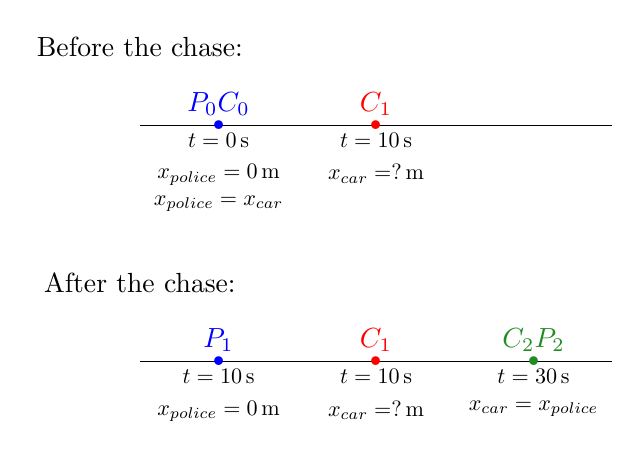
\begin{tikzpicture}
		\node at (-1, 4) {\text{Before the chase:}};
		\draw[] (-1, 3) -- (5, 3);

		\node[above, scale=1, color=blue] at (0, 3) (p) {$P_0C_0$};
		\node[above, scale=1, color=red] at (2, 3) (c) {$C_1$};

		\node[scale=3, color=blue] at (0, 3) (p1) {.};
		\node[scale=3, color=red] at (2, 3) (p2) {.};
		
		\node[below, scale=0.8] at (0, 3) (p) {$t=0\,\mathrm{s}$};
		\node[below, scale=0.8] at (2, 3) (c) {$t=10\,\mathrm{s}$};
		\node[below, scale=0.8] at (2, 3-0.4) (x) {$x_{car}=?\,\mathrm{m}$};
		\node[below, scale=0.8] at (0, 3-0.4) (x) {$x_{police}=0\,\mathrm{m}$};
		\node[below, scale=0.8] at (0, 3-0.8) (x) {$x_{police}=x_{car}$};

		\node at (-1, 1) {\text{After the chase:}};
		\draw[] (-1, 0) -- (5, 0);

		\node[above, scale=1, color=blue] at (0, 0) (p) {$P_1$};
		\node[above, scale=1, color=red] at (2, 0) (c) {$C_1$};
		\node[above, scale=1, color=ForestGreen] at (4, 0) (x) {$C_2P_2$};

		\node[scale=3, color=blue] at (0, 0) (p1) {.};
		\node[scale=3, color=red] at (2, 0) (p2) {.};
		\node[scale=3, color=ForestGreen] at (4, 0) (p3) {.};
		
		\node[below, scale=0.8] at (0, 0) (p) {$t=10\,\mathrm{s}$};
		\node[below, scale=0.8] at (0, -0.4) (x) {$x_{police}=0\,\mathrm{m}$};
		\node[below, scale=0.8] at (2, 0) (c) {$t=10\,\mathrm{s}$};
		\node[below, scale=0.8] at (2, -0.4) (x) {$x_{car}=?\,\mathrm{m}$};
		\node[below, scale=0.8] at (4, 0) (x) {$t=30\,\mathrm{s}$};
		\node[below, scale=0.8] at (4, -0.4) (x) {$x_{car}=x_{police}$};
	\end{tikzpicture}
	\end{center}
    \end{figure}

	We can even take a closer look by roughly graphing the positions of the car with 
	respect to time:
	\begin{center}
		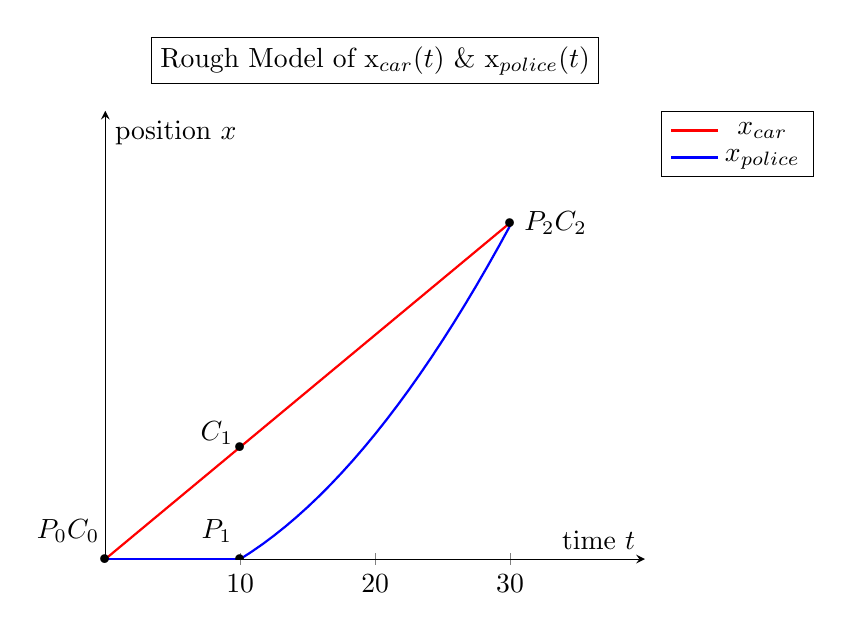
\begin{tikzpicture}
			\begin{axis}
				[
					domain=0:40,
					xmin=0,
					xmax=40,
					ymax=40,
					axis lines=center,
					legend pos=outer north east,
					title=$\boxed{\text{Rough Model of }\x_{car}(t)\text{ \& }\x_{police}(t)}$,
					xlabel=time $t$,
					ylabel=position $x$,
					xtick={0, 10, 20, 30},
					ytick,
				]
				\addplot[no marks, thick, domain=0:30, color=red] {x};
				\addlegendentry{$x_{car}$};
				\addplot[no marks, thick, domain=0:10, color=blue] {0};
				\addplot[no marks, thick, domain=10:30, color=blue] {(1/26.9)*(x-10)*(x+10)};
				\addlegendentry{$x_{police}$};

				\node[scale=3] at (30, 30) (x) {.};
				\node[right of=x, xshift=-12] {$P_2C_2$};
				\node[scale=3] at (10, 10) (x1) {.};
				\node[left of=x1, xshift=20, yshift=5] {$C_1$};
				\node[scale=3] at (10, 0) (x2) {.};
				\node[left of=x2, xshift=20, yshift=10] {$P_1$};
			\end{axis}
				\node[scale=3] at (0, 0) (x3) {.};
				\node[left of=x3, xshift=15, yshift=10] {$P_0C_0$};
		\end{tikzpicture}
	\end{center}

	From the graph, we can see that the speeding car moves for the entirety of the chase whereas
	the police car only begins to move $10$ seconds into the chase. We can also see that both cars 
	are at the same position at time $t=0$ and $t=30$, and so this will be our reference position. 
	As a result, we will set $t_2=30$ for both cars, but $t_1=0$ for the speeding car and $t_1=10$
	for the police car.
	
	Since the positions of both cars are equal at $t_2$, we can say that:
	\[\x_{car}(t_2) = \x_{police}(t_2) \]
	Now, while we know that $t_2=30$, we still need a expression for each function.

	\paragraph{The Police Car} In order define $\x_{police}(t)$, we need to integrate the velocity
	of the police car, however we do not have a velocity. Thus, we have to integrate acceleration to 
	get velocity, and we are given a constant acceleration of $a=10$:

	\begin{subequations}
	\begin{align}
		\vel_{car}(t) &= \int_{t_1}^{t} a \,\mathrm{d}t \\
		\vel_{car}(t) &= \int_{t_1}^{t} 10\,\mathrm{d}t \\
		\vel_{car}(t) &= [10(t) + C] - [10(t_1) + C]\\
		\vel_{car}(t) &= 10(t) - 10(10)\\
		\vel_{car}(t) &= 10t - 100 \\
	\end{align}
	Now to derive the function for position:
	\begin{align}
		\x_{car}(t) &= \int_{t_1}^{t} \vel_{car}(t)\,\mathrm{d}t \\
		\x_{car}(t) &= \int_{t_1}^{t} 10t - 100 \,\mathrm{d}t \\
		\x_{car}(t) &= [10\frac{(t)^2}{2}-100t+C] - [10\frac{(t_1)^2}{2}-100t+C] \\
		\x_{car}(t) &= [10\frac{(t)^2}{2}-100t] - [10\frac{(10)^2}{2}-100(10)]\\
		\x_{car}(t) &= 5t^2-100t - (-500)\\
		\x_{car}(t) &= 5t^2 - 100t + 500 \\
	\end{align}

	\paragraph{The Speeding Car} We will have to integrate velocity to derive a function
	for the speeding car's position, however while we do not know the value of its velocity,
	we can just take the integral of a constant:
	\begin{align}
		\x_{car}(t) &= \int_{t_1}^{t} v_{car} \\
		\x_{car}(t) &= t\cdot v_{car} - t_1\cdot v_{car} \\
		\x_{car}(t) &= t\cdot v_{car} - (0)\cdot v_{car} \\
		\x_{car}(t) &= t\cdot v_{car}
	\end{align}

	\newpage
	Now to set the two functions equal to each other at $t=t_2=30$:
	\begin{align}
		\x_{car}(30) &= \x_{police}(30) \\
		30\cdot v_{car} &= 5(30)^2 - 100(30) + 500 \\
		30\cdot v_{car} &= 2000 \\
		\Rightarrow v_{car} &= \frac{2000}{30} \\
		&\boxed{v_{car} = \frac{200}{3} \,\mathrm{m/s}}
	\end{align}	
	\end{subequations}
	Thus, the velocity of the speeding car was $\frac{200}{3}\,\mathrm{m/s}$.
\end{document}
>>>>>>> d277412f89eca5cb34333aae26b914d8e28252a6
